\documentclass[../main.tex]{subfiles}

\begin{document}
\section{Methods}
	
	\subsection{Participants}
	% Also mention pilot briefly
	
	
	\subsection{Questionnaire}
	To measure the aesthetic experience of each participant, we used a shortened version of the Aesthetic Experience Questionnaire \parencite[AEQ;][]{wanzerExperiencingFlowViewing2020}. We chose this questionnaire based on a number of factors. First of all, the theoretical background of an aesthetic flow experience \parencite{csikszentmihalyi1990art} seems intuitively relevant to our experiment design where participants will be exposed to a large number of images with varying aesthetic qualities. Second, this questionnaire seems fitting because the AEQ is supposed to be very generalizable to all visual aesthetic experiences and not only famous pieces in a museum. Finally, we picked the AEQ because the authors suggest that it should be possible to reduce the items on the six scales and still end up with a sufficient measurement of aesthetic experience.
	
	As the experience one has with art was not the primary focus of our study, we only used the highest loading items from each of the six scales, resulting in a total of six items at the start of our study in order to save time. Each item was presented with a five-point Likert scale, ranging from 0 (\textit{Strongly disagree}) to 4 (\textit{Strongly agree}). To test whether this shortened version of the AEQ was sufficient to explain the latent aesthetic experience, we used confirmatory factor analysis (CFA).
	
	
	
	\subsection{Behavioral Experiment}
	To determine whether GANalyze \parencite{goetschalckxGANalyzeVisualDefinitions2019} can be used to study what it means for an image to be aesthetic, I conducted a study to test whether human participants indeed preferred the images that GANalyze generated to be more aesthetic over a corresponding base image.
	
	I used GANalyze with AestheticsNet \parencite{kongPhotoAestheticsRanking2016} as the assessor and BigGAN-256 \parencite{brockLargeScaleGAN2019} pretrained on ImageNet \parencite{russakovskyImageNetLargeScale2015} as the generator to train the GANalyze model for 400,000 iterations. The training resulted in GANalyze being able to produce image sequences based on 1,000 ImageNet categories. For each ImageNet category, I generated three different seeds (i.e., three different images of Siamese cats) to test for an effect of category. Within each seed, GANalyze produced 21 images with a supposedly increasing amount of aesthetic value (Figure ~\ref{fig:sample_sequence}). I picked a broad range of $\alpha$-values with increasing density close to zero to obtain stimuli with obvious changes (e.g., $\alpha$ = 0.25), but also subtle changes (e.g., $\alpha$ = 0.0025). I chose these values because I hypothesized the participants to agree with GANalyze 100 of the time for trials with a large $\alpha$-value, and 50 of the time (picking at random) for very small $\alpha$-values, resulting in a psychometric function. The specific $\alpha$-values were chosen based on the results of a pilot study with a very broad range.
	
	\begin{figure}[ht]
		\caption{Truncated Sample of an Image Sequence from One Seed Produced by GANalyze}
		\label{fig:sample_sequence}
		\centering
		\begin{subfigure}{.18\textwidth}
			\centering
			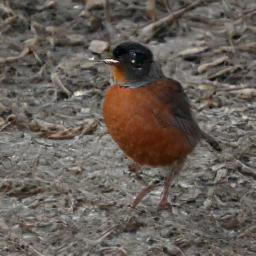
\includegraphics[width=1\linewidth]{methods/1}
			\caption{\centering $\alpha = -0.25$}
		\end{subfigure} \hfill
		\begin{subfigure}{.18\textwidth}
			\centering
			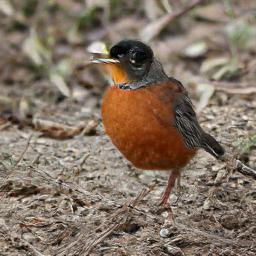
\includegraphics[width=1\linewidth]{methods/2}
			\caption{\centering $\alpha = -0.10$}
		\end{subfigure} \hfill
		\begin{subfigure}{.18\textwidth}
			\centering
			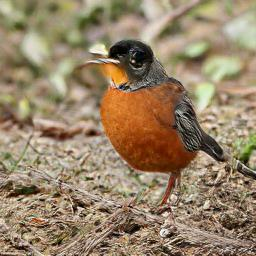
\includegraphics[width=1\linewidth]{methods/3}
			\caption{\centering $\alpha = 0$}
		\end{subfigure} \hfill
		\begin{subfigure}{.18\textwidth}
			\centering
			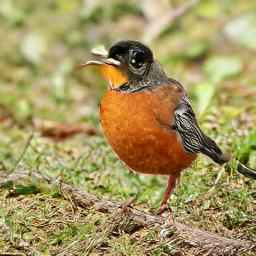
\includegraphics[width=1\linewidth]{methods/4}
			\caption{\centering $\alpha = 0.10$}
		\end{subfigure} \hfill
		\begin{subfigure}{.18\textwidth}
			\centering
			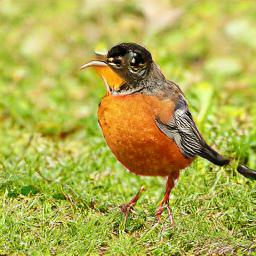
\includegraphics[width=1\linewidth]{methods/5}
			\caption{\centering $\alpha = 0.25$}
		\end{subfigure} \hfill
	\end{figure}
	
	489 ImageNet categories were manually excluded from the stimulus set because they either contained human faces (which are deliberately warped by BigGAN) or insects such as spiders which might make some participants feel uncomfortable. In addition, stimuli that were unrecognizable were also excluded. This resulted in 9xx categories, each with three seeds and 21 $\alpha$-values, equaling a total of \totalstimuli{} stimuli.
	
	The study was hosted on Prolific.co to obtain a large number of data points in a simple online task, ensuring each of the \totalstimuli{} stimuli was evaluated 2-3 times on average. Individuals younger than 17 or those without normal or corrected-to-normal vision were not allowed to participate. At the start of the study, participants were asked to fill in demographic details such as their age, gender, and country. They were also polled on their previous experience and familiarity with visual arts. Afterwards, they had to read and accept an informed consent document after which they were provided with instructions for the task.
	The participants carried out a spatial two-alternatives forced choice (2AFC) task in which they had to indicate which of the two presented GAN-generated images they considered to be most aesthetically pleasing. They did this by pressing "F" for the left, and "J" for the right image (Figure ~\ref{fig:trial_sequence}).
	
	Each trial consisted of two images generated from the same seed within an ImageNet category. One of the two images was always the base image with $\alpha = 0$ from that trial’s seed while the comparison image was, according to GANalyze at least, either more aesthetic ($\alpha > 0$) or less aesthetic ($\alpha < 0$). The $\alpha$-value for the comparison image differed for each trial, leading to differences in similarity between the base and comparison images for each trial. An $\alpha$-value close to zero indicates high similarity and, consequently, difficulty to discriminate between the images. An $\alpha$-value much larger or smaller than zero indicates low similarity and therefore easy discrimination. The position of the base and comparison image was randomized for each trial to prevent possible confounding factors. Each 10-minute block was created to contain a roughly uniform distribution of chosen $\alpha$-values and ImageNet categories to ensure that each participant is presented with a comparable stimulus set. Furthermore, the same category never appeared more than one time in a block.
	
	After 10 minutes, the task automatically turned to a screen thanking the participants for their assistance, after which they were given monetary compensation of £1.38 converted to their local currency.
	
	
	\begin{figure}
		\centering
		\caption{Example of a Sequence of Trials in the Study}
		\label{fig:trial_sequence}
		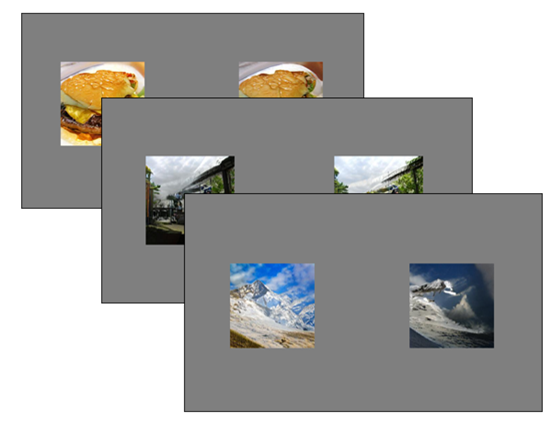
\includegraphics[scale=0.60]{trial_sequence}
	\end{figure}

	
	\subsection{Data Analysis}
	\subsubsection{Structural Equation Modeling}
	The first requirement for the model is that the latent variable measuring aesthetic experience was properly explained, In addition, we wanted to know whether age, sex, and nationality affect this. Furthermore, we are interested in the effects of aesthetic experience, age, sex, and nationality on the outcome variable of the behavioral task measured by percentage of agreeing with the neural network. To test this, we used structural equation modeling (SEM) with the \texttt{lavaan} package \parencite{rosseel2012lavaan} in R version 4.1.0 \parencite{rcoreteamlanguage} to build and evaluate models based on theory that would give an explanation to the data. All models were fitted using a maximum likelihood estimation method and the fits were evaluated with the comparative fit index (CFI), Tucker-Lewis index (TLI), and the root mean square error of approximation (RMSEA).
	
	First of all, we performed a priori CFA to validate whether our shortened version of the AEQ was indeed sufficient in explaining the latent aesthetic experience variable. We used the `emotional', `cultural', `perceptual', `understanding', `flow-proximal', and `flow-experience' scales as indicators for our latent variable. 
	
	Next, we moved on to more complicated structural models to better describe the full dataset. More specifically, we created a multiple indicators multiple causes (MIMIC) model aimed to show whether age, sex, and nationality affected the latent aesthetic experience variable. Crucially, we were interested in the effects of the aesthetic experience latent variable and age, sex, and nationality on the outcome of the image comparison behavioral task. We used the proportion of agreement with the GAN as the measure for aesthetic judgement here. Our initial idea for this model consisted of the latent variable, explained by the indicators, affecting aesthetic judgement in the behavioral task. Age, sex and nationality would have an effect on both the latent variable and the behavioral outcome of judgement. We also made another alternative model based on different theoretical arguments. For this second model, we decided that it did not make sense for nationality to have a direct effect on aesthetic judgement, so we removed that effect and instead added an effect of nationality on the cultural scale from the AEQ, as we believed this would make sense. These models would additionally test the questions \textcite{wanzerExperiencingFlowViewing2020} had regarding their homogeneous population sample. 
	
	Even though the new model MIMIC did not appear to be significantly better than the older one, we decided to keep the newer model as it made more theoretical sense.
	
	
	
	\subsubsection{Behavioral Task}
	Outliers, total participants, etc.
	
	(Merge with SEM perhaps)
	

\end{document}
